%========== Document settings ==========
\documentclass[11pt,a4paper,twoside,openany]{report}
\setlength\textwidth{145mm}
\setlength\textheight{247mm}
\setlength\oddsidemargin{14.2mm}
\setlength\evensidemargin{0mm}
\setlength\topmargin{0mm}
\setlength\headsep{0mm}
\setlength\headheight{0mm}
\let\openright=\cleardoublepage

%========== Language settings ==========
\usepackage[main=british,czech]{babel}
\usepackage[utf8]{inputenc}
\usepackage[T1]{fontenc}

%========== Packages =============
\usepackage{stddoc}
\usepackage{circuitikz}

%========== Date format ===============
\newdateformat{monthyeardate}{\monthname[\THEMONTH] \THEYEAR}

%========== Declaration ==========
\newcommand\declarationpage{\clearpage
\vspace*{\fill}
\noindent\textbf{Declaration}\\[0.25cm]
I declare that I completed the presented thesis independently and that all used sources are quoted in accordance with the Methodological instructions that cover the ethical principles for writing an academic thesis.\\
\hrule\vspace*{1cm}

\noindent\textbf{Prohlášení}\\[0.25cm]
\foreignlanguage{czech}{Prohlašuji, že jsem předloženou práci vypracoval samostatně a že jsem uvedl veškeré použité informační zdroje v souladu s Metodickým pokynem o dodržování etických principů při přípravě vysokoškolských závěrečných prací.}\\
\begin{center}
	\begin{minipage}{0.45\textwidth}
		\begin{flushleft}
			V Praze, \hdashrule{3cm}{0.5pt}{2pt}
		\end{flushleft}
	\end{minipage}
	~
	\begin{minipage}{0.45\textwidth}
		\begin{flushright}
			\noindent\begin{tabular}{c}
				\\
				\hdashrule{4cm}{0.5pt}{2pt}\\
				Martin Šimák
			\end{tabular}
		\end{flushright}
	\end{minipage}
\end{center}
\clearpage}

%========== Acknowledgements ==========
\newcommand\acknowledgementspage{\clearpage
\vspace*{\fill}
\noindent\textbf{Acknowledgements}\\[0.25cm]
First and foremost, I would like to thank my supervisor, Jiří Velebil, for his outstanding guidance and his zeal throughout the creation of this thesis. Further, I would like to thank my family and my colleagues, namely Erik Rapp and Karolína Veselá, for their invaluable support.\\
\hrule\vspace*{1cm}

\noindent\textbf{Poděkování}\\[0.25cm]
\foreignlanguage{czech}{Především bych rád poděkoval svému vedoucímu, Jiřímu Velebilovi, za jeho vynikající vedení a za jeho zapálenost a vstřícnost během tvorby této práce. Dále bych rád poděkoval své rodině a svým kolegům, zejména Eriku Rappovi a Karolíně Veselé, za jejich neocenitelnou podporu.}
\clearpage}

%========== Abstract ==========
\newcommand\abstractpage{\clearpage
\noindent\textit{Title:}\\
\textbf{Connections on Differentiable Manifolds}\\[0.25cm]
\textit{Author:} Martin Šimák\\[0.25cm]
\textit{Study programme:} Open Electronic Systems\\[0.25cm]
\textit{Supervisor:} doc. RNDr. Jiří Velebil, Ph.D., Department of Mathematics FEE\\[0.25cm]
\textit{Abstract:}\\
One of the aims of this thesis is to fully introduce a comprehensive differentiable structure on a smooth manifold. To achieve that, we first inspect various aspects of its definition. Further, we introduce a tangent structure on said manifolds, allowing us to locally speak of derivatives and vector fields. This construction naturally results in definitions of a covariant derivative and a connection form, where the former serves as a generalization of a derivative in a direction and the latter as a tool for ``glueing'' tangent spaces together. As a climax of the thesis, we show that the two previously mentioned additional structures on the ambient manifold are equivalent.\\[0.25cm]
\textit{Keywords:} smooth manifolds, tangent structure, covariant derivative, connection\\[0.5cm]
\noindent\textit{Název práce:}\\
\textbf{Konexe na diferencovatelných varietách}\\[0.25cm]
\textit{Autor:} Martin Šimák\\[0.25cm]
\textit{Studijní program:} Otevřené elektronické systémy\\[0.25cm]
\textit{Vedoucí:} doc. RNDr. Jiří Velebil, Ph.D., katedra matematiky FEL\\[0.25cm]
\textit{Abstrakt:}\\
\foreignlanguage{czech}{Jedním z cílů této práce je v plném měřítku uvést rozsáhlou diferenciální strukturu na hladké varietě. Abychom toho dosáhli, prozkoumáme nejprve jednotlivé aspekty její definice. Dále na varietách uvedeme tečnou strukturu, jenž nám umožňuje lokálně hovořit o derivacích a vektorových polích. Tato konstrukce přirozeně vyúsťuje v definice kovariantní derivace a konexe, přičemž první z pojmů slouží jakožto zobecnění derivace ve směru a druhý jakožto nástroj pro \uv{slepování} tečných prostorů. Jako vyvrcholení práce ukážeme, že tyto dvě dodatečné struktury na varietě jsou ekvivalentní.}\\[0.25cm]
\textit{Klíčová slova:} hladké variety, tečná struktura, kovariantní derivace, konexe\\[0.5cm]
\clearpage}

%========== Draft settings ==========
\usepackage{lipsum}


\makeindex
\begin{document}

    \pagenumbering{gobble}
    
    %========== Title page ==========
    % Suppress displaying the page number on the title page + count the following page as page 1 (not used)
    \begin{titlepage}
        % Define a new command for horizontal lines, change thickness here
\newcommand{\HRule}{\rule{\linewidth}{0.5mm}}
\center

%========== Header ==========
\textsc{\LARGE Czech Technical University in Prague,\\Faculty of Electrical Engineering}\\[1.5cm]
\textsc{\Large B2MPROJ6 - Thesis project}\\[0.5cm]
% \textsc{\Large Master's thesis}\\[0.5cm]

%========== Title ==========
\HRule\\[0.6cm]
{\huge\bfseries Inductive Wireless Power Transfer}\\[0.3cm] % Title of your document
\HRule\\[1.5cm]

%========== Authors ==========
\begin{minipage}{0.45\textwidth}
    \begin{flushleft}
        \large
        \textit{Author}\\
        M. \textsc{Šimák}\\
        \textsc{Department of Electromagnetic Field}
    \end{flushleft}
\end{minipage}
~
\begin{minipage}{0.45\textwidth}
    \begin{flushright}
        \large
        \textit{Supervisor}\\
        Ing. J. \textsc{Kraček}, Ph.D.\\
        \textsc{Department of Electromagnetic Field}
    \end{flushright}
\end{minipage}

%========== Logo ==========
% Position at 3/4 of the screen
\vfill\vfill\vfill

\includegraphics[width=0.3\textwidth]{src/ctu_logo_black.jpg}

%========== Date ==========
\vfill\vfill
{\large\monthyeardate\today}
% Push the date up 1/4 of the remaining page
\vfill
    \end{titlepage}

    %========== Blank page ==========
    \newpage\blankpage

    % %========== Assignment ==========
    % 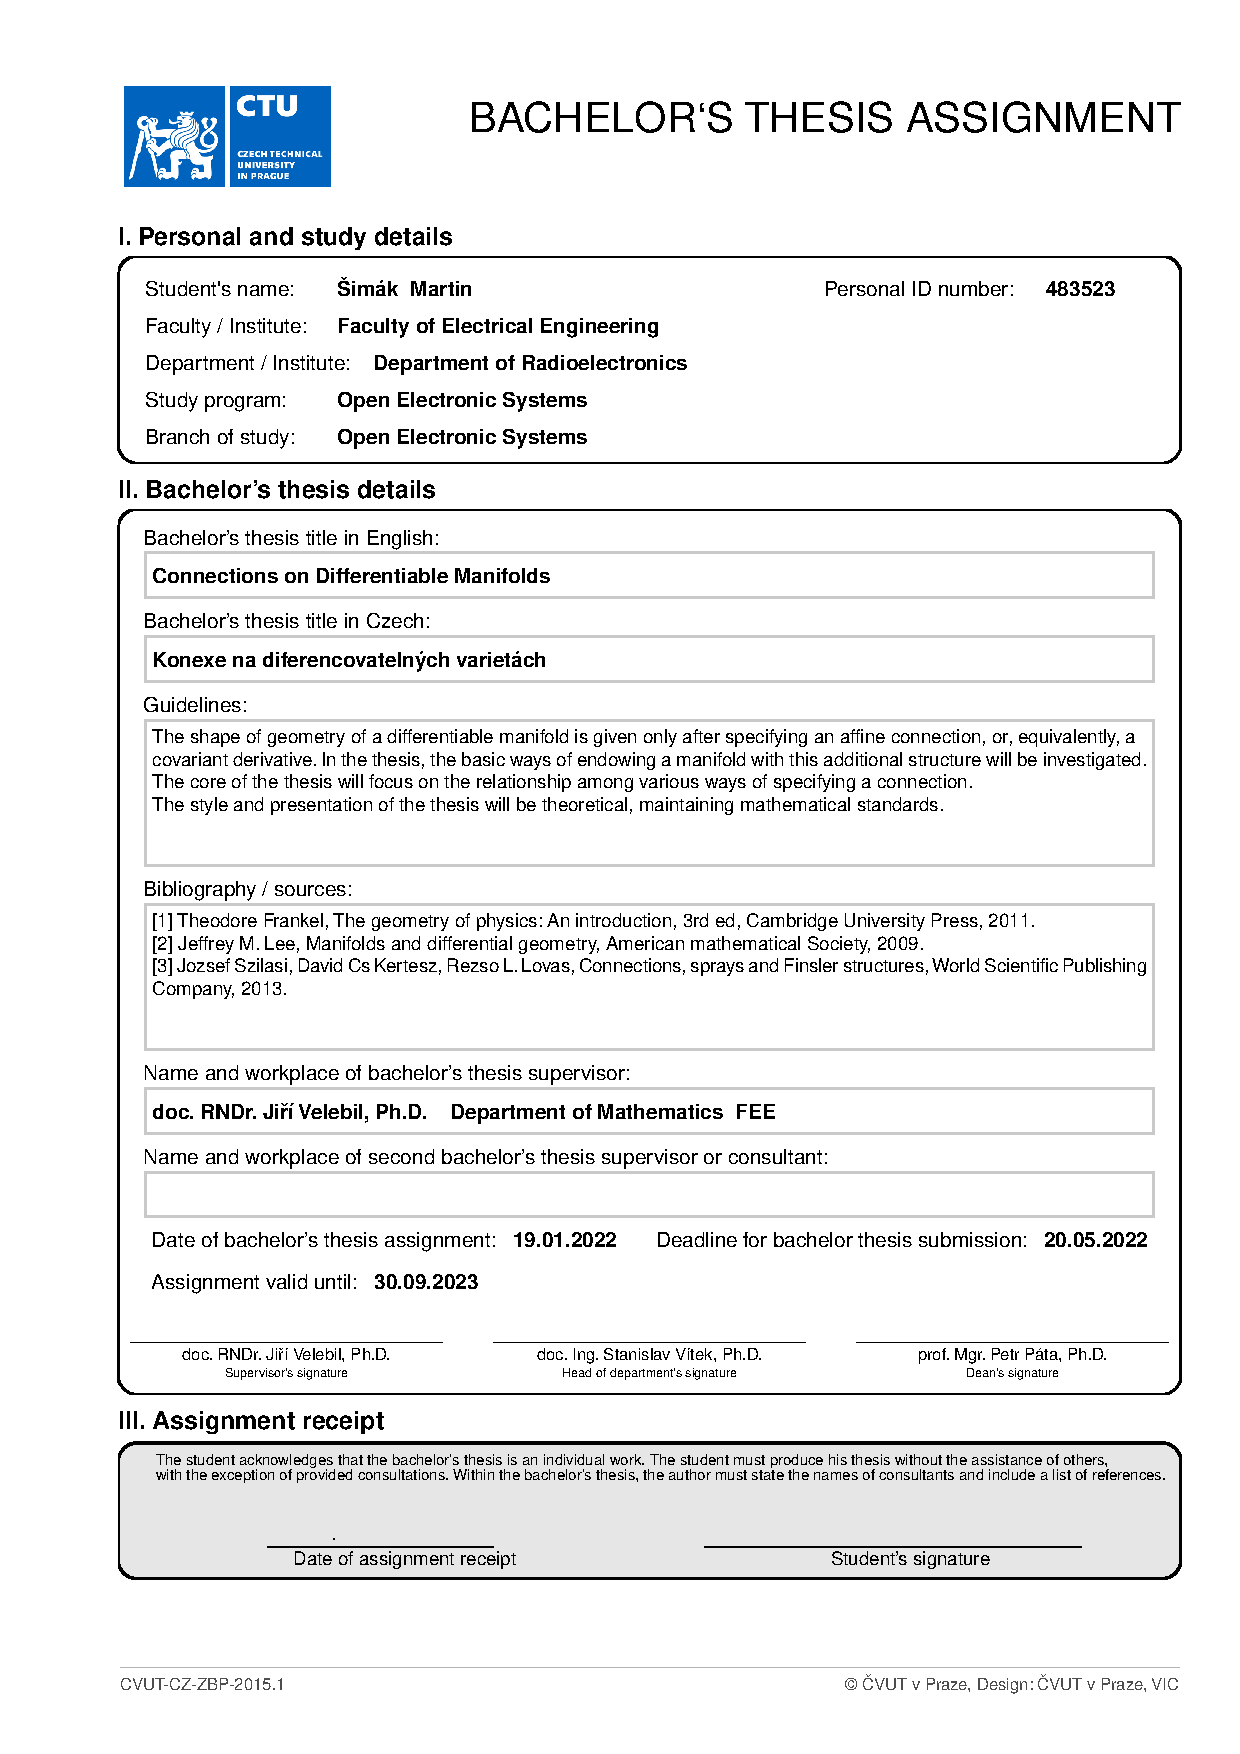
\includepdf[pages=-]{src/assignment.pdf}

    % %========== Blank page ==========
    % \newpage\blankpage

    % Start counting pages in roman numerals
    \pagenumbering{roman}

    % %========== Declaration ==========
    % \declarationpage

    % %========== Acknowledgements ==========
    % \acknowledgementspage

    % %========== Abstract ==========
    % \abstractpage

    % Start counting pages in arabic numerals
    \pagenumbering{arabic}

    %========== Table of contents ==========
    \tableofcontents

    %========== Introduction ==========
    % This is just a very vague introduction for the thesis project which is to be rewritten later on.
    \chapter*{Introduction}
    \label{chap:introduction}
    \addcontentsline{toc}{chapter}{\nameref{chap:introduction}}
    
    In recent years, the landscape of wireless power transfer (WPT) has undergone a significant transformation, fueled by the growing demand for convenient and efficient energy transfer methods in various industries. Among the plethora of wireless power transfer technologies, inductive wireless power transfer (IWPT) has emerged as a promising solution, particularly in the automotive sector. This project aims to delve into the fundamentals of inductive wireless power transfer, focusing on key aspects such as basic configuration, simulation of resistance and inductance, and a comparative analysis of simulation results against analytical formulas. The investigation also extends to the simulation of coils commonly employed in the automotive industry for mobile phone charging, utilizing exemplar coils provided by the esteemed collaboration with STMicroelectronics.

    The automotive industry is undergoing a paradigm shift towards electric vehicles (EVs) and the integration of advanced technologies. As vehicles become more electrified, the demand for efficient and seamless methods of charging electronic devices within the vehicle, such as mobile phones, has intensified. Inductive wireless power transfer, characterized by the transmission of energy through magnetic fields, has garnered attention for its potential to provide a convenient and cable-free charging experience. This project addresses the burgeoning need for a deeper understanding of IWPT systems, their design parameters, and their application in the automotive domain.

    \paragraph*{Synopsis of the thesis.} In \textbf{Chapter~\ref{chap:introduction-to-iwpt}}, we aim to explore the basic configuration of inductive wireless power transfer systems. This chapter also introduces the tools for analysis of IWPT systems, such as equivalent circuit models.

    \textbf{Chapter~\ref{chap:simulation-of-iwpt-systems}} conducts simulations of resistance and inductance using ANSYS Maxwell software, with a particular focus on zero frequency (DC) scenarios. Further on, we compare simulation results with analytical formulas to validate the accuracy and reliability of the simulation model.

    In conclusion, this thesis project represents a comprehensive investigation into the evolving field of inductive wireless power transfer, with a specific emphasis on its application within the automotive industry. The combination of theoretical exploration, simulation studies, and collaboration with industry leaders is poised to contribute valuable insights that will propel the advancement of wireless power transfer technologies in the automotive sector.

    \paragraph*{Methodology.} The research methodology involves a step-by-step exploration of inductive wireless power transfer, starting with a theoretical foundation and progressing to detailed simulations using ANSYS Maxwell software. The comparison of simulation results with analytical formulas will provide a rigorous validation process. Additionally, the project will leverage the expertise and resources of STMicroelectronics for the simulation and analysis of coils relevant to automotive applications.


    %========== Chapter 1: Introduction to inductive wireless power transfer ==========
    \chapter{Introduction to inductive wireless power transfer}
    \label{chap:introduction-to-iwpt}

    Chapter intro text\dots

    \section{Equivalent circuit analysis}

        Section intro text\dots

        % Parametrize, adjust horizontal and vertical distances, add coupling arrow, scale down
        \begin{figure}[!ht]
            \centering
            \begin{circuitikz}[american]
                % Source
                \draw (0,0) to[generic, l_=$X_{\mathrm{M}}$] (3,0)
                to[short] (4,0)
                to[generic, l_=$R_{\mathrm{S}}$] (6,0)
                to[L, l_=$L_{\mathrm{S}}$] (6,-3)
                to[short, -*] (0,-3);
                \draw (6.2,-2.3) node {$\bullet$};
                % Voltage arrow
                \draw[-Latex] (0,-0.2) -- (0,-2.8) node[midway,right] {$U_{\mathrm{S}}$};
                % Current arrow
                \draw[-Latex] (2,-0.7) arc[start angle=120,delta angle=-330,x radius = 2,y radius = 1];
                \draw (1.5,-1.5) node {$I_{\mathrm{S}}$};
                % Power lost
                \draw[-Latex] (5,0.3) -- (6,1.3) node[midway,above left] {$P_{\mathrm{S}}$};
                % Matching network block
                \draw (-0.3,-3.3) rectangle +(3.3,4);
                \node[below] at (-0.3+0.5*3.3,-3.3) {MN};
                % Coupling element block
                \draw (3.1,-3.3) rectangle +(3.5,4);
                \node[below] at (3.1+0.5*3.5,-3.3) {CE};
                % Source + FC block
                \draw (-1.5,-3.3) rectangle +(1,4);
                \node[rotate=90] at (-1.5+0.5*1,-3.3+0.5*4) {Source + FC};
                \draw (-1.5+1,0) to[short] (0,0);
                \draw (-1.5+1,-3) to[short] (0,-3);
                \draw[dashed] (-1.5+1+0.1,-3.3) to (-1.5+1+0.1,1.3);
                % Power supplied
                \draw[-Latex] (-1.5+0.5*1,1.1) -- (-1.5+1+0.1,1.1) node[at start,left] {$P_{\mathrm{T}}$};
                % Side of source block
                \draw (-1.9,-4) rectangle +(8.7,5.5);
                \node[below] at (-1.9+0.5*8.7,-4) {Side of source};

                % Appliance
                \draw (8,0) to[generic, l_=$R_{\mathrm{A}}$] (10,0)
                to[short] (12,0)
                to[generic, l_=$Z_{\mathrm{L}}$] (12,-3)
                to[short] (8,-3)
                to[L, l_=$L_{\mathrm{A}}$] (8,0);
                \draw (7.8,-2.3) node {$\bullet$};
                % Current arrow
                \draw[-Latex] (9.5,-0.7) arc[start angle=120, delta angle=-330, x radius = 1, y radius = 1];
                \draw (9.5,-1.5) node {$I_{\mathrm{A}}$};
                % Power lost
                \draw[-Latex] (9,0.3) -- (10,1.3) node[midway,above left] {$P_{\mathrm{A}}$};
                % Coupling element block
                \draw (7.5,-3.3) rectangle +(2.5,4);
                \node[below] at (7.5+0.5*2.5,-3.3) {CE};
                % Complex load block
                \draw (10.1,-3.3) rectangle +(2.5,4);
                \node[below] at (10.1+0.5*2.5,-3.3) {CL};
                % Side of appliance block
                \draw (7.3,-4) rectangle +(5.5,5.5);
                \node[below] at (7.3+0.5*5.5,-4) {Side of appliance};
            \end{circuitikz}
            \caption{\label{fig:circuit}Circuit}
        \end{figure}

        \begin{figure}[!ht]
            \centering
            \resizebox{\textwidth}{!}{%
            \begin{circuitikz}[american,>=Latex]
                % Parameters
                \def\ComponentLength{3}
                \def\ComponentHeight{.5}
                \def\CircuitXMargin{.5}
                \def\CircuitYMargin{.5}
                \def\SourceFCWidth{1}
                \def\SourceLoopXRadius{2}
                \def\SourceLoopYRadius{1}
                \def\InnerBlockHeight{2*\CircuitYMargin+\ComponentLength}
                \def\InnerBlockXMargin{.4}
                \def\InnerBlockYMargin{.7}
                \def\InnerBlockGap{.2}
                \def\OuterBlockGap{.5}

                % Source + FC block
                \draw (\InnerBlockXMargin,\InnerBlockYMargin) rectangle ++(\SourceFCWidth,\InnerBlockHeight);
                \node[anchor=center,rotate=90] at (\InnerBlockXMargin+.5*\SourceFCWidth,\InnerBlockYMargin+\CircuitYMargin+.5*\ComponentLength) {Source + FC};
                \draw[dashed] (\InnerBlockXMargin+\SourceFCWidth+.5*\InnerBlockGap,0) -- ++(0,2*\InnerBlockYMargin+\InnerBlockHeight);
                \draw[->] (\InnerBlockXMargin+.5*\SourceFCWidth,1.5*\InnerBlockYMargin+\InnerBlockHeight) -- ++(.5*\SourceFCWidth+.5*\InnerBlockGap,0) node[at start, left] {$P_{\mathrm{T}}$};
                % Source circuit
                \node (SourceCircuitBottomLeft) at (\InnerBlockXMargin+\SourceFCWidth+\InnerBlockGap+\CircuitXMargin,\InnerBlockYMargin+\CircuitYMargin) {};
                \node (SourceCircuitBottomRight) at (\InnerBlockXMargin+\SourceFCWidth+2*\InnerBlockGap+3*\CircuitXMargin+2*\ComponentLength,\InnerBlockYMargin+\CircuitYMargin) {};
                \node (SourceCircuitCentre) at (\InnerBlockXMargin+\SourceFCWidth+1.5*\InnerBlockGap+2*\CircuitXMargin+\ComponentLength,\InnerBlockYMargin+\CircuitYMargin+.5*\ComponentLength) {};
                \draw ($(SourceCircuitBottomLeft)-(\InnerBlockGap+\CircuitXMargin,0)$)
                    to[short, -*] ++(\InnerBlockGap+\CircuitXMargin,0)
                    to[short] ++(\ComponentLength+\CircuitXMargin+\InnerBlockGap+\CircuitXMargin+\ComponentLength,0)
                    to[L, l^=$L_{\mathrm{S}}$, mirror] ++(0,\ComponentLength)
                    to[generic, l^=$R_{\mathrm{S}}$] ++(-\ComponentLength,0)
                    to[short] ++(-2*\CircuitXMargin-\InnerBlockGap,0)
                    to[generic, l^=$X_{\mathrm{M}}$] ++(-\ComponentLength,0)
                    to[short, *-] ++(-\CircuitXMargin-\InnerBlockGap,0);
                \draw (SourceCircuitBottomRight)+(.5*\ComponentHeight,.2*\ComponentLength) node {$\bullet$};
                % Source voltage arrow
                \draw[<-] (SourceCircuitBottomLeft) -- ++(0,.95*\ComponentLength) node[midway, right] {$U_{\mathrm{S}}$};
                % Loop current arrow
                \draw[-Latex] ($(SourceCircuitCentre)+({\SourceLoopXRadius*cos(120)},{\SourceLoopYRadius*sin(120)})$) arc[start angle=120,delta angle=-330,x radius = \SourceLoopXRadius,y radius = \SourceLoopYRadius];
                \draw ($(SourceCircuitCentre)+(-1.5,0)$) node {$I_{\mathrm{S}}$};
                % Active power lost
                \draw[->] ($(SourceCircuitBottomRight)+(-.5*\ComponentLength,\ComponentLength+.5*\ComponentHeight)$) -- ++(-.5*\ComponentHeight+\CircuitYMargin+.5*\InnerBlockYMargin,-.5*\ComponentHeight+\CircuitYMargin+.5*\InnerBlockYMargin) node[at end, right] {$P_{\mathrm{S}}$};
                % Matching network block
                \draw ($(SourceCircuitBottomLeft)+(-\CircuitXMargin,-\CircuitYMargin)$) rectangle ++(2*\CircuitXMargin+\ComponentLength,\InnerBlockHeight);
                \node[below] at ($(SourceCircuitBottomLeft)+(.5*\ComponentLength,-\CircuitYMargin)$) {MN};
                % Coupling element block
                \draw ($(SourceCircuitBottomRight)-(\ComponentLength+\CircuitXMargin,\CircuitYMargin)$) rectangle ++(2*\CircuitXMargin+\ComponentLength,\InnerBlockHeight);
                \node[below] at ($(SourceCircuitBottomRight)-(.5*\ComponentLength,\CircuitYMargin)$) {CE};
                % Side of source block
                \draw (0,0) rectangle ++(2*\InnerBlockXMargin+\SourceFCWidth+2*\InnerBlockGap+4*\CircuitXMargin+2*\ComponentLength,2*\InnerBlockYMargin+2*\CircuitYMargin+\ComponentLength);
                \node[below] at (\InnerBlockXMargin+.5*\SourceFCWidth+\InnerBlockGap+2*\CircuitXMargin+\ComponentLength,0) {Side of source};

                % Appliance circuit
                \node (ApplianceCircuitBottomLeft) at ($(SourceCircuitBottomRight)+(2*\CircuitXMargin+2*\InnerBlockXMargin+\OuterBlockGap,0)$) {};
                \node (ApplianceCircuitBottomRight) at ($(ApplianceCircuitBottomLeft)+(2*\ComponentLength+2*\CircuitXMargin+\InnerBlockGap,0)$) {};
                \node (ApplianceCircuitCentre) at ($.5*(ApplianceCircuitBottomLeft)+.5*(ApplianceCircuitBottomRight)$) {};
                \draw (ApplianceCircuitBottomLeft)
                    to[short] ++(2*\ComponentLength+2*\CircuitXMargin+\InnerBlockGap,0)
                    to[generic, l_=$Z_{\mathrm{L}}$] ++(0,\ComponentLength)
                    to[short] ++(-\ComponentLength-2*\CircuitXMargin-\InnerBlockGap,0)
                    to[generic, l^=$R_{\mathrm{A}}$] ++(-\ComponentLength,0)
                    to[L, l^=$L_{\mathrm{A}}$, mirror] ++(0,-\ComponentLength);
                \draw (ApplianceCircuitBottomLeft)+(-.5*\ComponentHeight,.2*\ComponentLength) node {$\bullet$};
            \end{circuitikz}%
            }
            \caption{\label{fig:circuit2}Circuit2}
        \end{figure}


    %========== Chapter 2: Simulation of IWPT systems ==========
    \chapter{Simulation of IWPT systems}
    \label{chap:simulation-of-iwpt-systems}

    In the first chapter of this thesis, we introduce the concept of a smooth manifold. To readers experienced in topology, definition of the aforementioned might come across as trivial, but we consider it very important to specify how exactly we approach manifolds in general, since the underlying definitions might differ from text to text.

    Apart from the smooth manifold itself, we will also introduce other key concepts of differential topology, such as charts, atlases, paracompactness, etc.

    \section{Charts and atlases}

        Before we begin, let us discuss the goal of this section. We would like to introduce a structure on a set that endows it with the property of ``looking like'' $\mathbb R^n$ locally. In general, this will not be necessarily achievable globally on the whole set, but we will manage to arrive at a reasonable compromise using charts and atlases.

        \begin{definition}
            \index{chart}
            Let $M$ be a set. A \emph{chart} on $M$ is a pair $(U,\mathbf x)$ consisting of $U \subseteq M$ and an injective map $\mathbf x:U \to \mathbb R^n$ such that $\mathbf x[U] = \{\mathbf x(a) \mid a \in U\}$ is an open set in $\mathbb R^n$. The composite $x^i = \mathrm{pr}_i \circ \mathbf x: M \to \mathbb R$ is often called the \emph{$i$-th coordinate function}.
        \end{definition}
        
        \begin{note}
            Since $\mathbf x$, by definition, has $\R^n$ as a codomain, we can always write its action upon a point $p \in M$ as $\mathbf x: p \mapsto \mathbf x(p) = \big( x^1(p),\dots,x^n(p) \big)$. Whenever we wish to emphasize the individual coordinate functions, we write $\big( x^1,\dots,x^n \big)$ or $\big( x^i \big)$ instead of $\mathbf x$.
        \end{note}
        
        \begin{remark}
            Note that we have defined charts on a plain set $M$. Therefore, we do not require $U$ in $(U,\mathbf x)$ to be open since we do not have the topological structure on $M$ just yet.
        \end{remark}

    \section{Theoretical analysis}

        Some general talk\dots

        \subsection{Length of the coils}
            \paragraph{Underlying theorem.} Let $f$ be a function whose derivative is continuous on an interval $\alpha \leq \theta \leq \beta$. The arc length of the graph of $r=f(\theta)$ from $\theta=\alpha$ to $\theta=\beta$ is
            \begin{align}
                \l &= \int_\alpha^\beta \sqrt{|f(\theta)|^2 + |f'(\theta)|^2} \d\theta = \int_\alpha^\beta \sqrt{r^2 + \(\frac{\partial r}{\partial \theta}\)^2} \,\d\theta.
            \end{align}
            
            \paragraph{Application.} Since the \emph{radius change} of the created spirals is 1.46 mm per turn, we can write the following formulas for the spiral curves of the transmitting and receiving coils:
            \begin{align}
                r(\theta) &= 10+\frac{1.46}{2\pi} \theta, \quad 0 \leq \theta \leq N\cdot 2 \pi,
            \end{align}
            where $N$ is the number of turns of the respective coil. For such curves, we obtain
            \begin{align}
                \l_{\mathrm{TxSpiral}} &= \int_0^{10 \cdot 2\pi} \sqrt{\(10+\frac{1.46}{2\pi} \theta\)^2+\(\frac{1.46}{2\pi}\)^2} \d\theta\ \mathrm{mm},
            \\
                \l_{\mathrm{RxSpiral}} &= \int_0^{5 \cdot 2\pi} \sqrt{\(10+\frac{1.46}{2\pi} \theta\)^2+\(\frac{1.46}{2\pi}\)^2} \d\theta\ \mathrm{mm}.
            \end{align}
            These formulas can then be evaluated, e.g. using \emph{Wolfram Alpha}. The results are
            \begin{align}
                \l_{\mathrm{TxSpiral}} &= \SI{1087.1}{\milli\metre},
            &
                \l_{\mathrm{RxSpiral}} &= \SI{428.9}{\milli\metre}.
            \end{align}
            
            \paragraph{Result.} For the total length of a coil, the feeding terminals must be taken into account:
            \begin{align}
                \l_{\mathrm{TxTerminal1}} &= \SI{94.0}{\milli\metre},
            &
                \l_{\mathrm{RxTerminal1}} &= \SI{94.0}{\milli\metre},
            \\
                \l_{\mathrm{TxTerminal2}} &= \SI{86.7}{\milli\metre},
            &
                \l_{\mathrm{RxTerminal2}} &= \SI{79.5}{\milli\metre}.
            \end{align}
            Hence, the final length of the transmitting and receiving coils are
            \begin{align}
                \l_{\mathrm{Tx}} &= l_{\mathrm{TxSpiral}} + l_{\mathrm{TxTerminal1}} + l_{\mathrm{TxTerminal2}} = \SI{1.268}{\metre},
            \\
                l_{\mathrm{Rx}} &= l_{\mathrm{RxSpiral}} + l_{\mathrm{RxTerminal1}} + l_{\mathrm{RxTerminal2}} = \SI{0.602}{\metre}.
            \end{align}

        \subsection{DC resistance of the coils}
            The DC resistance $R$ of a wire of uniform cross-sectional area $A$, length $\l$ and resistivity $\rho = \sigma^{-1}$, where $\sigma$ is conductivity, can be calculated using the formula
            \begin{align}
                R &= \frac{\rho \l}{A} = \frac{\l}{\sigma A}.
            \end{align}

            We can apply this formula to our case of the aforementioned transmitting and receiving coils which consist of copper wire of cross-sectional area $A = \SI{1}{\milli\metre\squared}$. The conductivity of annealed copper is $\sigma = \SI{5.8001e7}{\siemens\per\metre}$. Altogether, we obtain the values of DC resistance
            \begin{align}
                R_{\mathrm{Tx}} &= \frac{1.268}{5.8001 \cdot 10^7 \cdot 1 \cdot 10^{-6}} = \SI{21.9}{\milli\ohm},
            \\
                R_{\mathrm{Rx}} &= \frac{0.602}{5.8001 \cdot 10^7 \cdot 1 \cdot 10^{-6}} = \SI{10.4}{\milli\ohm}.
            \end{align}
            These results, compared with the simulation results of $R_{\mathrm{Tx}} = \SI{21.7}{\milli\ohm}$ and $R_{\mathrm{Tx}} = \SI{10.5}{\milli\ohm}$, verify the computational credibility of \emph{ANSYS Maxwell}.
    

    % %========== Bibliography ==========
	% \newpage
	% \begin{thebibliography}{20}
	% 	\bibitem{cartan:differential-calculus} Henri Cartan, \emph{Differential calculus}, Hermann, 1983.
		
	% 	\bibitem{dieudonne:treatise-on-analysis} Jean Dieudonn\'{e}, \emph{Treatise on analysis}, volume 3, Academic Press, 1972.
		
	% 	\bibitem{engelking:general-topology} Ryszard Engelking, \emph{General topology}, Heldermann, Berlin, 1989.
		
	% 	\bibitem{frankel:the-geometry-of-physics-an-introduction} Theodore Frankel, \textit{The geometry of physics: an introduction}, 3rd ed, Cambridge University Press, 2011.
		
	% 	\bibitem{gauld:nonmetrisable-manifolds} David Gauld, \emph{Non-metrisable manifolds}, Springer, Singapore, 2014.
		
	% 	\bibitem{hartman:orginary-differential-equations} Philip Hartman, \emph{Ordinary differential equations}, John Wiley \& Sons, New York, 1964.
		
	% 	\bibitem{lee:manifolds-and-differential-geometry} Jeffrey M. Lee, \emph{Manifolds and differential geometry}, volume 107, American Mathematical Society, Rhode Island, 2009.
		
	% 	\bibitem{lee:intro-to-smooth-manifolds} John M. Lee, \emph{Introduction to smooth manifolds}, Springer, New York, 2012.
		
	% 	\bibitem{lucyshyn-wright:on-geometric-noton-of-connection-and-its-expression-in-tangent-categories} Rory B. B. Lucyshyn-Wright, On the geometric notion of connection and its expression in tangent categories, \emph{Theory Appl. Categ.} 33 (2018), 832-866. \url{http://www.tac.mta.ca/tac/volumes/33/28/33-28.pdf}, Accessed: \monthyeardate\today.
		
	% 	\bibitem{rosicky:abstract-tangent-functors} Jiří Rosický, Abstract tangent functors, \emph{Diagrammes} 12 (1984): JR1-JR11. \url{http://eudml.org/doc/91746}, Accessed: \monthyeardate\today.
		
	% 	\bibitem{szilasi-kertesz-lovas:connections-sprays-and-finsler-structures} J\'{o}zsef Szilasi, D\'{a}vid Cs Kert\'{e}sz, Rezs\H{o} L. Lovas, \emph{Connections, sprays and Finsler structures}, World Scientific Publishing
	% 	Company, 2013.
		
	% \end{thebibliography}
	
    % %========== Index ==========
	% \printindex

\end{document}
